% Created 2024-06-16 Sun 00:13
% Intended LaTeX compiler: pdflatex
ocumentclass[10pt]{article}% =================================BASE====================================%
\documentclass[10pt]{report}
\usepackage[left=2cm,right=2cm,top=2cm,bottom=2cm]{geometry} % Marges
\usepackage[T1]{fontenc} % Nécessaire avec FrenchBabel
\usepackage[utf8]{inputenc} % Important pour symboles Francophones, é,à,etc
\usepackage{csquotes} % Recommandé par PDFLatex lors de la compilation. 


% Calligraphie
%\usepackage{lmodern} % Ça, ça set latin modern
%\usepackage{mathrsfs} %Permet la command \mathscr (Lettres attachées genre) \mathscr(B)

% Calligraphie
%\usepackage{pxfonts} % Met le texte ET les maths en Palatino + donne accès à des symboles math
\usepackage{palatino} % Cette commande met seulement le texte en police palatino
\usepackage{lmodern} % Pour les maths?
% Use lmodern for sans-serif
\usepackage{mathrsfs} % Permet la command \mathscr (Lettres attachées genre) \mathscr(B)





% Bibliographie
%\usepackage[backend=bibtex,style=phys,sorting=ynt]{biblatex}
\usepackage[backend=biber,sorting=ynt,style=ieee]{biblatex}
\addbibresource{/home/charlesedouard/Desktop/Travail/Documentation/master-bibliography.bib}



\usepackage{amsmath, amssymb, amsthm} % Symb. math. (Mathmode+Textmode) + Beaux théorèmes.
\usepackage{mathtools,cancel,xfrac} % Utilisation de boîtes \boxed{} + \cancelto{}{}, xfrac
\usepackage{graphicx, wrapfig} % Géstion des figures.
\usepackage{hyperref} % Permettre l'utilisation d'hyperliens.
\usepackage{color} % Permettre l'utilisation des couleurs.
\usepackage{colortbl} % Color tables
\usepackage[dvipsnames]{xcolor} % Couleurs avancées.
\usepackage{titling} % Donne accès à \theauthor, \thetitle, \thedate

% Physique
\usepackage{physics} % Meilleur package pour physicien. 


% Style
\usepackage{lipsum} % For fun
\usepackage{tikz} % Realisation de figures TIKZ.
\usepackage{empheq} % Boite autour de MULTIPLE équations
\usepackage{bbding}

% Français
\usepackage[french]{babel} % Environnements en Français.
% ==============================BASE-(END)=================================%



% ================================SETTINGS=================================%
% Pas d'indentation en début de paragraphe :
\setlength\parindent{0pt}
\setlength{\parskip}{0.15cm}

% Tableaux/tabular
% Espace vertical dans les tabular/tableaux
\renewcommand{\arraystretch}{1.2}
% Couleur des tableaux/tabular
\rowcolors{2}{violet!5}{}

% Couleurs de hyperliens :
\definecolor{mypink}{RGB}{147, 0, 255}
\hypersetup{colorlinks, 
             filecolor=mypink,
             urlcolor=mypink, 
             citecolor=mypink, 
             linkcolor=mypink, 
             anchorcolor=mypink}


\usepackage{titling} % Donne accès à \theauthor, \thetitle, \thedate

% Physique
\usepackage{physics} % Meilleur package pour physicien. 


% Style
\usepackage{lipsum} % For fun
\usepackage{tikz} % Realisation de figures TIKZ.
\usepackage{empheq} % Boite autour de MULTIPLE équations

% Français
\usepackage[french]{babel} % Environnements en Français.
% ==============================BASE-(END)=================================%





% ================================SETTINGS=================================%
% Pas d'indentation en début de paragraphe :
\setlength\parindent{0pt}
\setlength{\parskip}{0.15cm}

% Tableaux/tabular
% Espace vertical dans les tabular/tableaux
\renewcommand{\arraystretch}{1.2}
% Couleur des tableaux/tabular
\rowcolors{2}{violet!5}{}

% Couleurs de hyperliens :
\definecolor{mypink}{RGB}{147, 0, 255}
\hypersetup{colorlinks, 
             filecolor=mypink,
             urlcolor=mypink, 
             citecolor=mypink, 
             linkcolor=mypink, 
             anchorcolor=mypink}


% Numéros d'équations suivent les sections :
\numberwithin{equation}{section} 

% Les « captions » sont en italique et largeur limitée
\usepackage[textfont = it]{caption} 
\captionsetup[wrapfigure]{margin=0.5cm}

% Retirer l'écriture en gras dans la table des matières
\usepackage{tocloft}
\renewcommand{\cftsecfont}{\normalfont}
\renewcommand{\cftsecpagefont}{\normalfont}

% Change bullet style
\usepackage{pifont}
\usepackage{enumitem}
%\setlist[itemize,1]{label=\ding{224}}
\setlist[itemize,1]{label=\ding{239}}
\renewcommand{\boxtimes}{\blacksquare}
% ================================SETTINGS=================================%



% ==============================NEWCOMMANDS================================%

% Vecteurs de base :
\newcommand{\nvf}{\vb{\hat{n}}}
\newcommand{\ivf}{\vb{\hat{i}}}
\newcommand{\jvf}{\vb{\hat{j}}}
\newcommand{\kvf}{\vb{\hat{k}}}
\newcommand{\uu}{\vb{u}}
\newcommand{\vv}{\vb{v}}
\newcommand{\ust}{\vb{u}_{\ast}}

% Physics empty spaces 
\newcommand{\typical}{\vphantom{A}}
\newcommand{\tall}{\vphantom{A^{x^x}_p}}
\newcommand{\grande}{\vphantom{\frac{1}{xx}}}
\newcommand{\venti}{\vphantom{\sum_x^x}}
\newcommand{\pt}{\hspace{1pt}} % One horizontal pt space

% Moyenne numérique entre deux points de grilles. 
\newcommand{\xmean}[1]{\overline{#1}^x}
\newcommand{\ymean}[1]{\overline{#1}^y}
\newcommand{\zmean}[1]{\overline{#1}^z}
\newcommand{\xymean}[1]{\overline{#1}^{xy}}

% Tilde over psi
\newcommand{\tpsi}{\tilde{\psi}}
\newcommand{\tphi}{\tilde{\phi}}

% Nota Bene env : (\ding{89})
%\newcommand{\nb}{$\boxed{\text{\footnotesize\EightStarConvex}\pt \mathfrak{N. B.}}$\hspace{4pt}}
\newcommand{\nb}{\underline{{\footnotesize\EightStarConvex}\pt $\mathfrak{N.B.}$\vphantom{p}}\hspace{3pt}}


% Define the nota bene environment
\usepackage{tcolorbox}
\newtcolorbox{notabene}{
     colback=blue!5,
     colframe=black,
     boxrule=0.5pt,
     arc=2pt,
     left=5pt,
     right=5pt,
     top=5pt,
     bottom=5pt,
}


\newcommand{\cmark}{\ding{52}}
\newcommand{\xmark}{\ding{55}}
% ==============================NEWCOMMANDS================================%



% ==============================PAGE-TITRE=================================%
% Titlepage 
\newcommand{\mytitlepage}{
\begin{titlepage}
\begin{center}
{\Huge Contrat Été 2023 \par}
\vspace{2cm}
{\Huge \MakeUppercase{\thetitle} \par}
\vspace{2cm}
RÉALISÉ DANS LE CADRE\\ D'UN PROJET POUR \par
\vspace{2cm}
{\Huge ISMER--UQAR \par}
\vspace{2cm}
{\thedate}
\end{center}
\vfill
Rédaction \\
{\theauthor}\\
\url{charles-edouard.lizotte@uqar.ca}\\
ISMER-UQAR\\
Police d'écriture : \textbf{CMU Serif Roman}
\end{titlepage}
}
% ==============================PAGE-TITRE=================================%



% =================================ENTÊTE==================================%
\usepackage{fancyhdr}
\pagestyle{fancy}
\setlength{\headheight}{13pt}
\renewcommand{\headrulewidth}{0.025pt} % Ligne horizontale en haut

\fancyhead[R]{\textit{\thetitle}}
\fancyhead[L]{\ \thepage}
\fancyfoot[R]{\textit{\theauthor}}
\fancyfoot[L]{}
\fancyfoot[C]{} 
% =================================ENTÊTE==================================%
\author{Charles-Édouard Lizotte}
\date{07/03/2023}
\title{Rapport hebdomadaire -- McGill}
\hypersetup{
 pdfauthor={Charles-Édouard Lizotte},
 pdftitle={Rapport hebdomadaire -- McGill},
 pdfkeywords={},
 pdfsubject={},
 pdfcreator={Emacs 27.1 (Org mode 9.6.7)}, 
 pdflang={French}}
\begin{document}

\mytitlepage
\tableofcontents\newpage


\section{{\bfseries\sffamily DONE} Débugger le modèle \emph{shallow water} à 2 et 3 couches [1/1]}
\label{sec:orgfab7af9}
\subsection{Workflow}
\label{sec:org05a5f55}
Commençons par relancer le modèle pour 5 ans à seulement deux couches.
De la manière que j'ai tout recodé, il ne suffit qu'à redéfinir le nombre de couches \emph{nz} à 2 et \emph{H2} à 3000 mètres.
Les gravités réduites ont été formulées de sorte à retrouver la même vitesse pour les ondes barocliniques \(c_{bc}\).
En détail, à deux couches
\begin{equation}
g_2' = c_{bc} \qty(\frac{H_1+H_2}{H_1H_2}) = g \qty(\frac{\Delta \rho_{1,2}}{\rho_1}),
\end{equation}
Donc il est assez simple d'imposer un différentiel de \(\rho\) entre les couches, dans le but de fixer la vitesses des ondes barocliniques.

\textbf{N.B.} Après quelques heures/journées de travail, j'ai trouvé des erreurs, mais pas les miennes.
En gros, la \emph{thickness} était calculée entre deux pas de temps différents.
Faudrait en glisser un mot à Tianze sur son \emph{git}.
C'est fait, mais David m'a mentionné que Tianze ne risque malheureusement pas de répondre.

\subsection{{\bfseries\sffamily DONE} Rencontre avec David}
\label{sec:org033a4d5}
J'ai rencontré david pour lui parler du problème, j'ai quelques indices personnels qui pourraient expliquer la convergence dans la zonne anti-cyclonique. 
Selon lui, c'est normal en \emph{shallow water} ce genre de truc.
Comme j'avais remarqué, en \emph{SW}, il y a une \emph{feedback loop} entre l'épaisseur de la couche supérieure et la valeur du forçage.
\begin{equation}
\text{Si } h \downarrow
\Rightarrow \tau (h) \uparrow
\Rightarrow u(\tau) \uparrow
\Rightarrow -\divergence(\vb{u}h) \uparrow
\end{equation}

Aussi, faut pas oublier que la vorticité et le courant se font advecter.
C'est probablemet de l'auto-advection et je capotais probablement pour rien, ça reste à voir ça.\\[0pt]

En gros, David a remarqué que j'avais initialement du bruit dans mes premières simulations mais pas dans les simulations subséquentes à 2 et trois couches.
Personnellement, je ne croyais pas que c'était un enjeu, considérant qu'il y a souvent du bruit numérique et que les instabilités barocliniques finissent toujours par arriver de toute manière.
Bref, David m'a convaincu du contraire : ça prend beaucoup de temps pour que ces instabilités finissent par émerger.
J'ai donc reparti les simulations numériques avec le même bruit qu'avant (de l'ordre de \(\mathcal{O}(0.1)\)).
Les résultats étaient identiques, j'en déduis donc qu'il faut absolument \textbf{toujours} un peu de bruits.

\subsection{Test à trois couches}
\label{sec:orgd486283}
Comme David l'a conseillé, on peut fait un simple test où les trois couches ont la même épaisseur et le même \(\Delta \rho_{k,k-1}\).
Ainsi les rayons de déformation sont données par des multiples du rayon de déformation du premier mode.
Les paramètres de l'expérience sont affichés dans le tableau suivant.
Les diagrammes de Hovmoler et les snapshot sont affichés en annexe de ce rapport.

\begin{table}[htbp]
\caption{\label{tab:org9f86e29}Valeur des différents paramètres de l'expérience de \notecite{chen_2021}, mais à 3 couches.}
\centering
\begin{tabular}{lll}
\hline
\hline
Paramètres & Symbole & Valeur\\[0pt]
\hline
Taille du domaine & L\textsubscript{x} = L\textsubscript{y} & 2000 km\\[0pt]
Pas de temps & \(\Delta\) t & 360 s\\[0pt]
Paramètre de Coriolis & f & 7\texttimes{}10\textsuperscript{-5} s\textsuperscript{-1}\\[0pt]
Amplitude du vent & \(\tau\)\textsubscript{atm} & 0.1 N m\textsuperscript{-2}\\[0pt]
Coefficient de viscosité biharmonique & A\textsubscript{bh} & dx\textsuperscript{4} \texttimes{}10\textsuperscript{-5} s\textsuperscript{-1}\\[0pt]
Coefficient de frottement au fond & r\textsubscript{drag} & 10\textsuperscript{-7} s\textsuperscript{-1}\\[0pt]
Coefficient dissipation du Laplacien inverse & r\textsubscript{InvLap} & (2\(\pi\)/L\textsubscript{y})\textsuperscript{2} \texttimes{} 10\textsuperscript{-6} s\textsuperscript{-1}\\[0pt]
Épaisseur de la couche en surface & H\textsubscript{1} & 1000 m\\[0pt]
Épaisseur de la seconde couche & H\textsubscript{2} & 1000 m\\[0pt]
Épaisseur de la couche au fond & H\textsubscript{3} & 1000 m\\[0pt]
Densité de l'eau (première couche) & \(\rho\)\textsubscript{1} & 1.0000 kg/m\textsuperscript{3}\\[0pt]
Différence de densité entre les couches & \(\Delta \rho\) & \(\frac{\rho_1c_{bc}^2}{g}\qty(\frac{H_1+H_2}{H_1H_2})\)\\[0pt]
Vitesse des ondes internes (semi-obsolète) & c\textsubscript{bc} & 2 ms\textsuperscript{-1}\\[0pt]
Gravité réduite (seconde couche) & g\textsubscript{2}' & 8 \texttimes{} 10\textsuperscript{-2} m/s\textsuperscript{2}\\[0pt]
Gravité réduite (troisième couche) & g\textsubscript{3}' & 6 \texttimes{} 10\textsuperscript{-3} m/s\textsuperscript{2}\\[0pt]
\hline
\hline
\end{tabular}
\end{table}

\section{{\bfseries\sffamily DONE} Installer et gérer le compte Oxygen fournit pas McGill}
\label{sec:org875fbf7}
L'administration m'a crée un compte, il faudrait vérifier tout ça.

This is done using a ssh client (present on mac, linux and windows by default), please ssh to your assigned computer. Your computer name is the name on the sticker on the computer tower. (jet)
On m'a créé un compte AOS (\emph{Atmospheric and Oceanic Sciences}), donc à partir de maintenant, je peux me connecter partout, tant que je suis sur le réseau de l'université McGill.
Le VPN ne marchera pas tant que les problèmes bureaucratiques ne seront pas réglé.\\[0pt]

Essentiellement, mon nom d'utilisateur est \emph{celizotte}, je peux me connecter au service \emph{Jump} en \emph{bash} à l'aide de la commande
\begin{verbatim}
ssh celizotte@jump.meteo.mcgill.ca
\end{verbatim}
et d'ici on peut se connecter sur Oxygen (le réseau à David?) à l'aide de la commande
\begin{verbatim}
ssh oxygen.meteo.mcgill.ca
\end{verbatim}

On m'a aussi fourni un ordinateur dénommé \emph{Jet}. Pour se connecter à Jet, il suffit d'utiliser la commande
\begin{verbatim}
ssh jet
\end{verbatim}
une fois connecté sur Jump. Il faudrait d'ailleurs que je demande à David où est l'ordinateur\ldots{} parce que je confirme qu'il n'est pas dans mon bureau.

\section{{\bfseries\sffamily DONE} Coder les mode barotropes et baroclines [3/3]}
\label{sec:org18d2b85}
\subsection{Rappel théorique : cas analytique du test à trois couches}
\label{sec:orgdb86d9c}
Étudions un cas facile pour se permettre de tester notre modèle numérique.
Assumons trois couches homogènes de 1000 mètres d'épaisseurs avec un différentiel de densité constant (Voir tableau \ref{tab:org126d81b}).

\begin{table}[htbp]
\caption{\label{tab:org126d81b}Tableau regroupant les paramètres de notre cas trivial.}
\centering
\begin{tabular}{lll}
\hline
\hline
Paramètre & Variable & Valeur\\[0pt]
\hline
Épaisseur 1ère couche & H\textsubscript{1} & H\textsubscript{tot}/3 = H\\[0pt]
Épaisseur 2ème couche & H\textsubscript{2} & H\textsubscript{tot}/3 = H\\[0pt]
Épaisseur 3ème couche & H\textsubscript{3} & H\textsubscript{tot}/3 = H\\[0pt]
Densité première couche & \(\rho\)\textsubscript{1} & \(\rho\)\textsubscript{1}\\[0pt]
Densité secondec couche & \(\rho\)\textsubscript{2} & \(\rho\)\textsubscript{1} + \(\Delta\) \(\rho\)\\[0pt]
Densité troisième couche & \(\rho\)\textsubscript{3} & \(\rho\)\textsubscript{1} + 2 \(\Delta\) \(\rho\)\\[0pt]
\hline
\hline
\end{tabular}
\end{table}

Aux dire de ce que nous avons découvert précédemment dans le dernier \href{rapport-2023-03-31.org}{rapport}, il est possible de créer une matrice représentant notre opérateur linéaire d'épaisseur à l'aide de la méthode des différences finies.
Rappellons que la surface fixe et le fond plat ajoutent des contraintes sur les premiers et derniers éléments de notre matrice, de sorte que 

\[
\mathcal{L}-\Lambda=\begin{pmatrix}
 F_{(1,2)} -\lambda_i & -F_{(1,2)} & 0 \\[0pt]
 -F_{(2,2)} & F_{(2,3)} + F_{(2,2)} - \lambda_i & -F_{(2,3)} \\[0pt]
 0 & -F_{(3,3)} & F_{(3,3)} -\lambda_i \\[0pt]
\end{pmatrix}
\]

Sachant que les \(g_j'\) dépendent de \(\Delta \rho_{(j,i)} = \rho_j - \rho_{j-1}\), on peut dire que \(g_2' = g_3' = g'\).
De plus, tous les \(H_i\) sont identiques, alors on peut simplifier les coefficient \(F\), ce qui se traduit mathématiquement par
\begin{equation}
F_{(i,j)} = \mathrm{F}\hspace{0.5cm} \forall\hspace{0.5cm} (i,j) : i,j \in \qty{1,2,3}
\end{equation}

On résoud le problème aux valeurs propres en trouvant le déterminant de cette matrice,
\begin{equation}
\label{eq:org4487fd9}
0 = (F-\lambda_i)\qty[(2F - \lambda_i)(F-\lambda_i) - F^2] - F^2(F-\lambda_i).
\end{equation}

L'équation \ref{eq:org4487fd9} se factorise, on retrouve donc
\begin{align}
&0 = (F-\lambda_i)\qty[(2F - \lambda_i)(F-\lambda_i) - 2F^2],\nonumber\\
&0 = (F-\lambda_i)\qty[(\lambda^2_i + 2F^2 - 3 F \lambda_i) - 2F^2],\nonumber\\
&0 = \lambda_i \qty(F-\lambda_i)\qty(\lambda_i - 3F).
\end{align}
Pour finir, nos valeurs propres sont données par
\begin{align}
\boxed{\hspace{0.4cm} \lambda_1 = 0,
\hspace{0.8cm} \lambda_2 = \frac{f_0^2}{g' H}, 
\hspace{0.8cm} \lambda_3 = \frac{3 f_0^2}{g'H}. \hspace{0.4cm}}   
\end{align}

\subsection{{\bfseries\sffamily DONE} Installer LAPACK}
\label{sec:org0460c2a}
Une fois internet revenu chez moi (grosse tempête de verglas), j'ai pu installer LAPACK,
\begin{verbatim}
sudo apt-get install libblas-dev liblapack-dev
\end{verbatim}
et pour trouver le \emph{path},
\begin{verbatim}
dpkg -L liblapack-dev
\end{verbatim}
ce qui nous permet d'ajouter
\begin{verbatim}
lapack_path=/usr/lib/x86_64-linux-gnu/lapack
\end{verbatim}
et de linker notre application Fortran avec
\begin{verbatim}
-lblas -L$lapack_path -llapack
\end{verbatim}

\subsection{{\bfseries\sffamily DONE} Implémenter l'algorithme pour trouver les valeurs propres}
\label{sec:org9edae80}
Consiste concrétement à recopier la matrice de l'opérateur linéaire du modèle QG de Louis-Philippe.
Il fallait juste faire très attention, parce qu'on définissait les gprime au plafond des couches et non au plancher.
Les fonctions \emph{F(i,j)} n'étaient donc pas les mêmes.
Une foit la matrice \emph{A} créée, on mettait tout ça dans la fonction SEEVG et le tour est joué.

\subsection{{\bfseries\sffamily DONE} Calculer les vorticités quasi-géostrophiques baroclines et barotropes}
\label{sec:orgcb0aa54}
À partir des fonctions de courant baroclines \(\psi_{BC}\), il est possible de retrouver des vorticité quasi-géostrophiques à l'aide de l'équation
\begin{equation}
q_{BT}^i = \laplacian \psi_{BT}^i + \Gamma^i \psi_{BT}^i,
\end{equation}
cité dans le code de Louis-Philippe.
Il faudrait donc implémenter ça, mais pour l'instant c'est en \emph{stand by} parce que les deux ont confirmé que ce n'était pas tant nécessaire.





\section{Annexe}
\label{sec:orgf9c1237}

\begin{figure}[htbp]
\centering
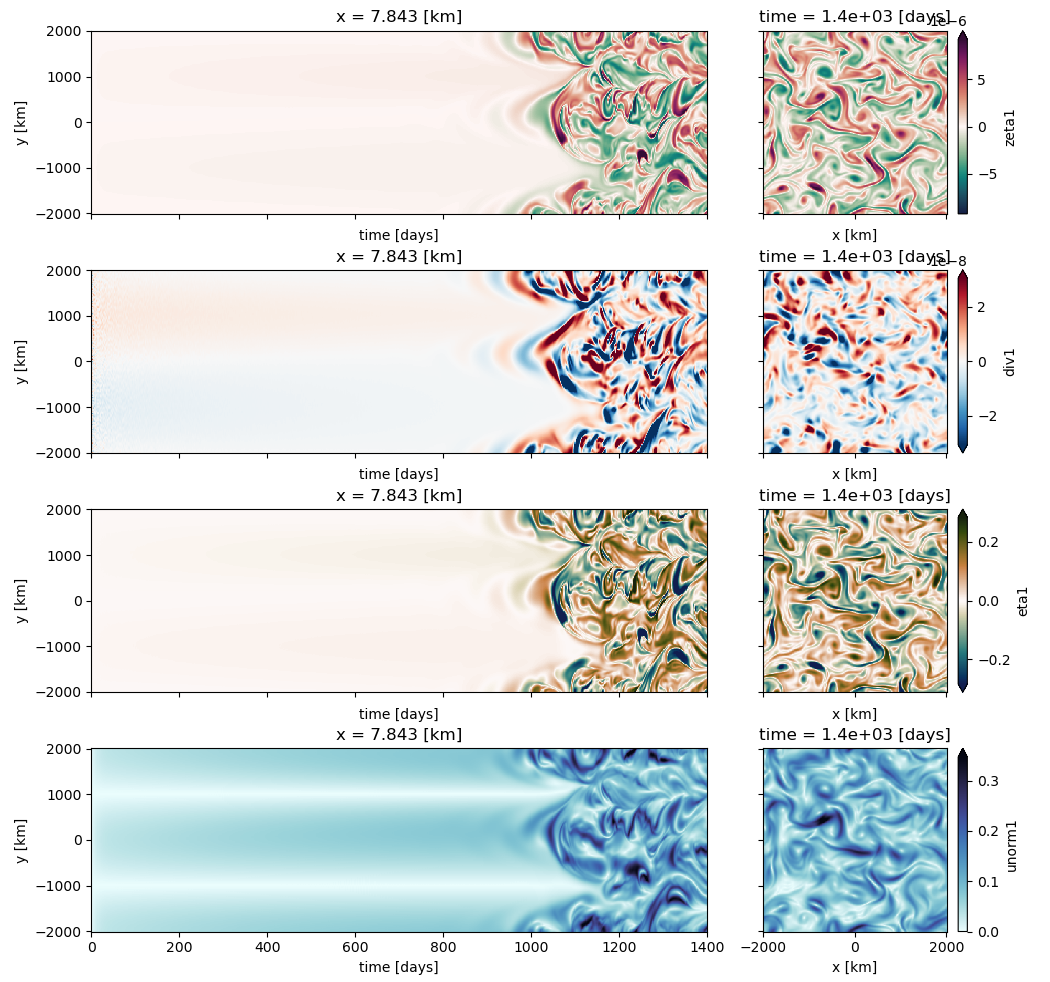
\includegraphics[width=.9\linewidth]{figures/tests/2023-04-08_test1.png}
\caption{\label{fig:org46999a9}Résultats du test à trois couches (Première couches)}
\end{figure}

\begin{figure}[htbp]
\centering
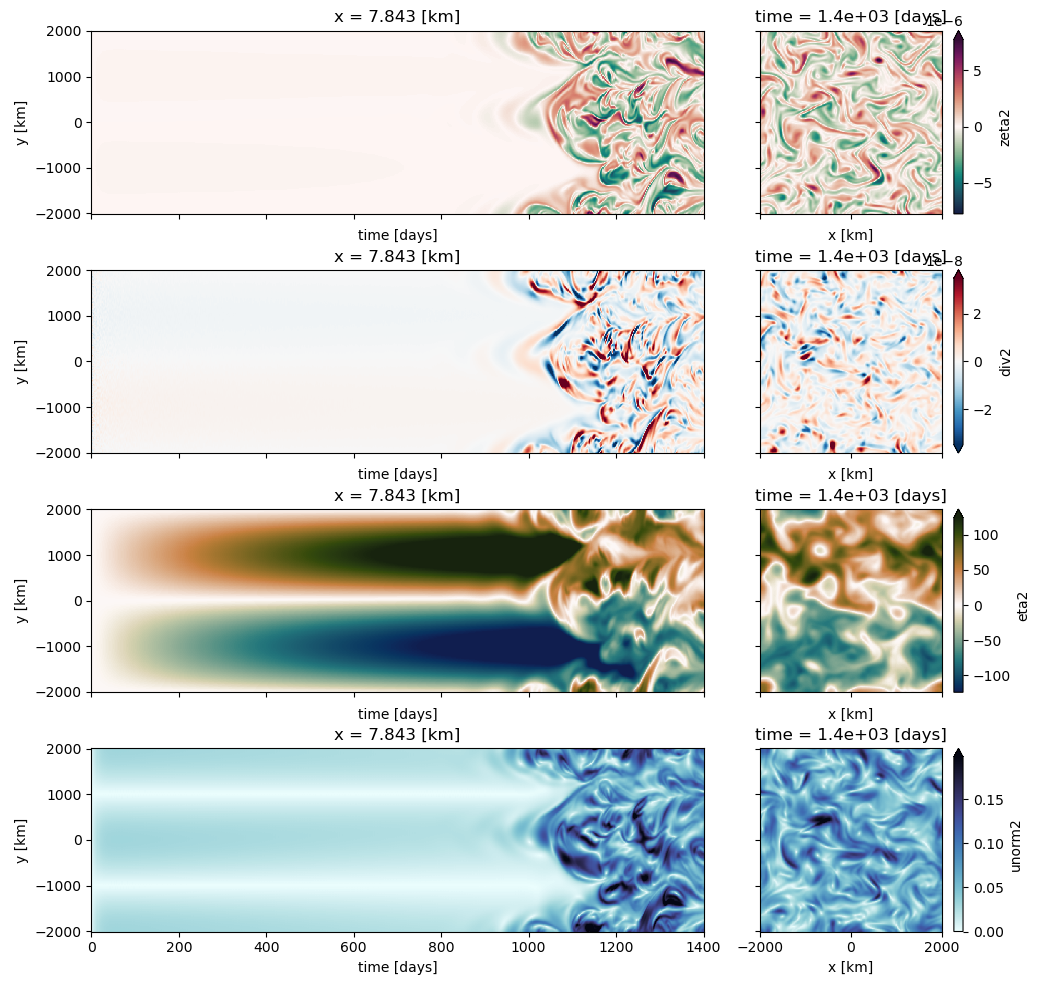
\includegraphics[width=.9\linewidth]{figures/tests/2023-04-08_test2.png}
\caption{Résultats du test à trois couches (Seconde couches)}
\end{figure}

\begin{figure}[htbp]
\centering
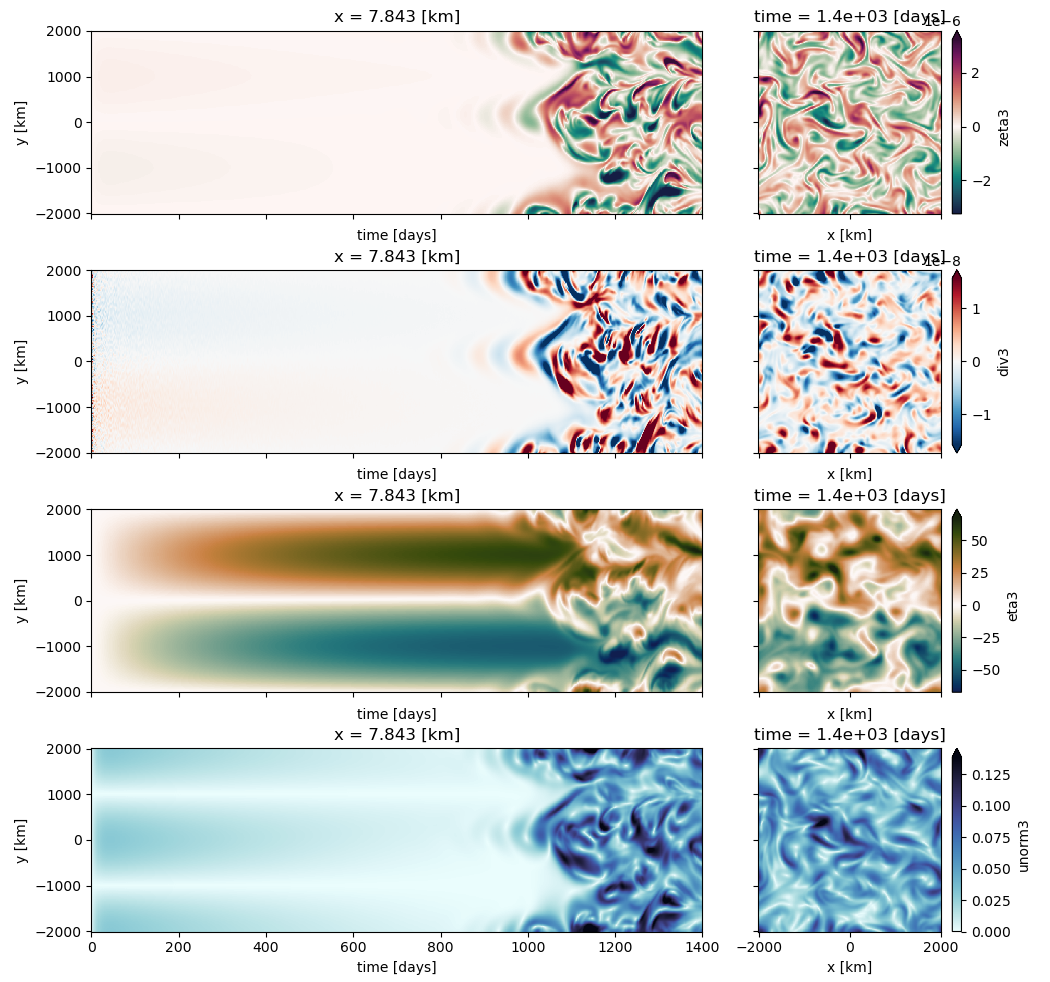
\includegraphics[width=.9\linewidth]{figures/tests/2023-04-08_test3.png}
\caption{Résultats du test à trois couches (Troisième couches)}
\end{figure}

\printbibliography
\end{document}